\documentclass[12pt]{article}

\usepackage{color}
\usepackage{graphicx}
\usepackage{amsmath}
\usepackage{float}
\usepackage{color}
\usepackage{indentfirst}
\usepackage{textcomp}
\usepackage{pifont}
\usepackage{multirow}
\usepackage{geometry}
\usepackage{algorithm}
\usepackage{algpseudocode}
\usepackage{amssymb}
\usepackage{algorithmicx}
\usepackage{amsmath} 
\usepackage{amsfonts}
\usepackage{bm}

\usepackage{listings}
\usepackage{xcolor}

\geometry{left = 2cm, right = 2cm, top = 3cm, bottom = 3cm}

\lstset{numbers=left,
        numberstyle=\tiny,
        keywordstyle=\color{blue}, 
        commentstyle=\color[cmyk]{1,0,1,0}, 
        frame=single, 
        escapeinside=``, 
        extendedchars=false, 
        xleftmargin=2em,xrightmargin=2em, aboveskip=1em, 
        tabsize=4, 
        showspaces=false 
       }

\floatname{algorithm}{Algorithm}
\renewcommand{\algorithmicrequire}{\textbf{Input:}}
\renewcommand{\algorithmicensure}{\textbf{Output:}}





\begin{document}

\vspace*{0.25cm}

\hrulefill

\thispagestyle{empty}

\begin{center}
\begin{large}
\sc{UM--SJTU Joint Institute \vspace{0.3em} \\ Bayesian Analysis \\ (VE414)}
\end{large}

\hrulefill

\vspace*{5cm}
\begin{Large}
\sc{{Assignment 2 \\ ~\\ }}
\end{Large}
\vspace{2em}

\end{center}


\vfill
\begin{large}

\begin{table}[h!]
\flushleft
\begin{tabular}{lll}
Name: Wu Guangzheng \hspace*{2em}\\
Student ID: 515370910014

\end{tabular}
\end{table}
\end{large}
\newpage
\begin{flushleft}


\section{Question 1} 

\qquad Consider the parameter of junior students is $p_j$ and the parameter of senior students is $p_s$. We first calculate the likelihood.

$$
L(p_j; x) = p^{S}(1-p)^{U}
$$

\qquad So the posterior should be

\vspace{-0.4cm}

\begin{align*}
f_{X\mid P_j}(x\mid p_j) &\propto f_{P_j \mid X}(p_j \mid x) \cdot f_{p_j}(p_j)\\
&\propto p_j^{S}(1-p)^{U} \cdot p^{3-1} (1-p)^{7-1}\\
&\sim \text{Beta}(19, 78)
\end{align*}

\qquad Similarly

$$
f_{X\mid P_s}(x\mid p_s) \sim \text{Beta}(37, 10)
$$

\qquad We plot these posteriors, with a label of $70/131$, which is the probability of a student to be enrolled

\begin{figure*}[h]
\centering
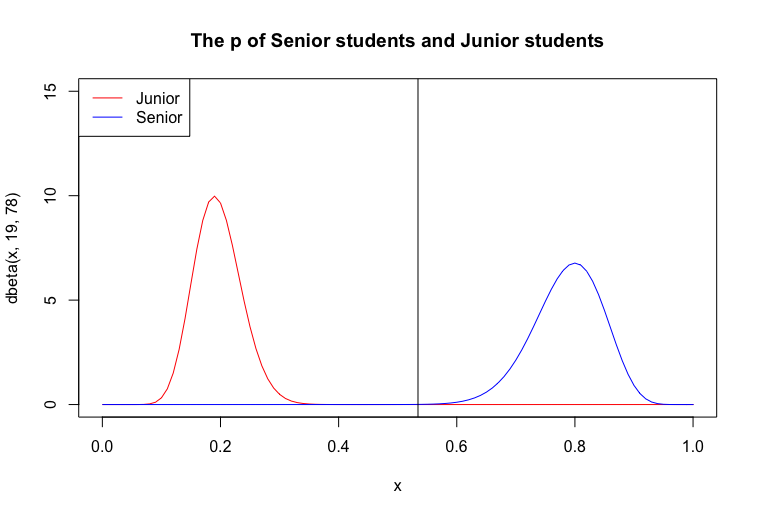
\includegraphics[width = 0.7\linewidth]{Q1.png}
\end{figure*}

\qquad From the graph, we can see that the probability for a junior student to be enrolled is much smaller than the $70/131$, while that of a senior student is much higher, which proves that the professor is guilty.

\newpage

\section{Question 2}

\subsection*{a)}

\qquad Since we know that it follows a Poisson distribution

$$
f_{P\mid X}(p\mid x) = \frac{y^xe^{-y}}{x!}
$$

\qquad So for the n data points, we have the likelihood,

$$
L(y; x) = \prod_{i=1}^n f_{P\mid X}(p\mid x) = \frac{y^{\sum_{i=1}^n X_i}e^{-ny}}{\prod_{i=1}^n x_i!}
$$

\qquad And we have the Gamma Distribution

$$
f_{Y}(y) = \frac{\beta^\alpha}{\Gamma(\alpha)} x^{\alpha-1}\exp (-\beta x)
$$

\qquad With calculation, 

$$
E[y] = \frac{\alpha}{\beta} = 15, \quad \text{Var}[y]= \frac{\alpha}{\beta^2} = 25 \qquad \longrightarrow \qquad  \alpha = 9, \quad \beta = 0.6
$$

\qquad So the prior should be 

$$
f_Y(y) \propto y^8 \exp(-0.6 y)
$$

\qquad So with these n data points, the posterior should be

$$
f_{Y\mid X}(y\mid x) \propto y^{\sum_{i=1}^n X_i + 8}e^{-(n+0.6)y}
$$

\qquad We can see that this is still a Gamma Distribution, with

$$
f_{Y\mid X}(y\mid x) \sim \text{Gamma}(\sum_{i=1}^n X_i + 9, n+0.6)
$$

\subsection*{b)}

\qquad According to the definition, the posterior predictive distribution should be

$$
f_{X^{*}\mid X}(x^{*}\mid x) = \int_{-\infty}^{\infty}f_{X^{*}\mid Y}(x^{*}\mid y) f_{Y \mid X}(y\mid x)dy
$$

\qquad The so consider the posterior calculated in question 1 as the prior for question 2, we are to find the prior predictive distriution for $X^{*}$, given a following prior

$$
f_{Y}(y) \sim \text{Gamma}(\sum_{i=1}^n X_i + 9, n+0.6)
$$

\qquad Besides, for the prior predictive distribution, we have

$$
p(y^{*}) = \frac{p(y\mid \theta)p(\theta)}{p(\theta\mid y)}
$$

\qquad So we have

$$
p(x^{*}) = \frac{\text{Possion}(y\mid x^{*})\cdot \text{Gamma}(x^{*}\mid \alpha, \beta)}{\text{Gamma}(x^{*}\mid \alpha + \sum_{i=1}^n X_i, \beta + n)}
$$

\qquad That is

$$
p(x^{*}) = \frac{\Gamma(\alpha + \sum X)\beta^{\alpha}}{\Gamma(\alpha)y!(\beta+n)^{\alpha + \sum X}}
$$

\qquad So

$$
p(x^{*}) \sim \text{Neg-Bin}(\alpha, \beta)
$$

\newpage

\section{Question 3}

\qquad Let's calculate the Jeffrey's prior first. Since it is a binominal distribution, 

$$
X_k \mid P \sim \text{Binominal}(k,p)
$$

\qquad So its likelihood should be 

$$
L(\theta; x) = c \cdot p^{\sum X_i} \cdot (1-p)^{(k - \sum X_i)}
$$

\qquad Where c is some function of $k$ but not of $p$

~\\

\qquad So we have the log likelihood

$$
l(\theta; x) = c +  \ln p \cdot \sum X_i + \ln (1-p) \cdot (k - \sum X_i) 
$$

\qquad We have $p$ as parameter, let $\bm{I}(\theta) = (I_{i,j}(\theta))_{1\times 1}$

$$
I(p) = E_{X\mid \theta}\left\{-\frac{\partial^2 l(\theta \mid x)}{\partial p^2} \right\} = E_{X\mid \theta} \left[ \frac{X}{p^2} + \frac{k - X}{(1-p)^2} \right]
$$

\qquad Since we know that the expectation of $X$ in a binominal distribution is $kp$, so

$$
I(p) = \frac{k}{p(1-p)}
$$

\qquad So the Jeffrey's prior should be 

$$
\pi(p) \propto p^{-1/2}(1-p)^{-1/2} \sim \text{Beta}(1/2, 1/2)
$$

\qquad We can see that for the Binominal distribution, the Jeffrey's prior is a beta function with $\alpha  = \frac{1}{2}$ and $\beta = \frac{1}{2}$.

~\\

\qquad Also we know that for a prior of $\text{Beta}(\alpha, \beta)$, if we have an observation of $X_k = n$, then the posterior should be $\text{Beta}(\alpha + n, \beta + k - n)$. Besides, for a uniform prior, it is just the same as the prior $\text{Beta}(1,1)$.

\newpage

\subsection*{a)}

\qquad Since we have $X_3 = 2$, then we have the posterior of these two are:

\vspace{-0.2cm}

\begin{table}[h]
\centering
\begin{tabular}{ll}
Uniform Prior & Beta(3,2)\\
Jeffrey's Prior & Beta(2.5, 1.5)
\end{tabular}
\end{table}

\qquad So we have the graph

\begin{figure*}[h]
\centering
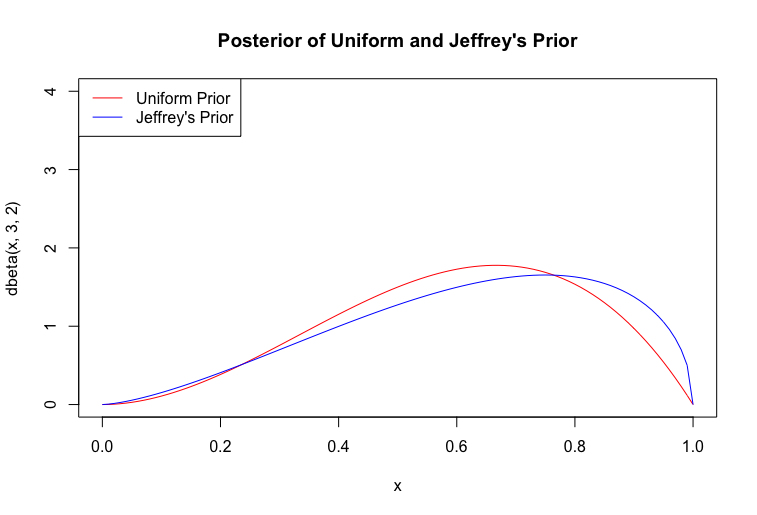
\includegraphics[width = 0.7\linewidth]{q3_1.png}
\end{figure*}

\qquad With code

\begin{lstlisting}[language=R]
    curve(dbeta(x, 3, 2), xlim = c(0,1), 
            ylim = c(0,4), col = "red")
    curve(dbeta(x, 2.5, 1.5), add = T, col = "blue")
    title(main = "Posterior of Uniform and Jeffrey's Prior")
    legend ( par('usr')[1], par('usr')[4], xjust = 0, 
            c('Uniform Prior', "Jeffrey's Prior"), 
            lwd = c(1, 1), lty = c(1, 1), 
            col = c('red', 'blue'))
\end{lstlisting} 

\newpage

\subsection*{b)}

\qquad Since we have $X_3 = 2$, then we have the posterior of these two are:

\vspace{-0.2cm}

\begin{table}[h]
\centering
\begin{tabular}{ll}
Uniform Prior & Beta(201,101)\\
Jeffrey's Prior & Beta(200.5, 100.5)
\end{tabular}
\end{table}

\qquad So we have the graph

\begin{figure*}[h]
\centering
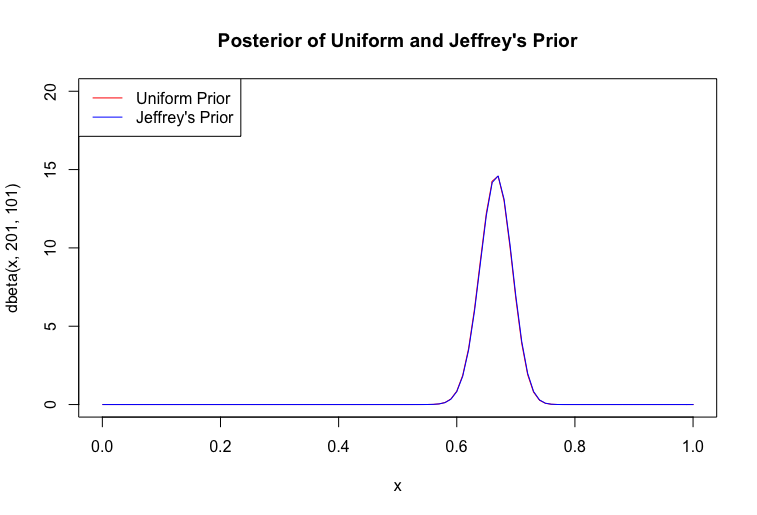
\includegraphics[width = 0.7\linewidth]{q3_2.png}
\end{figure*}

\qquad With code

\begin{lstlisting}[language=R]
    curve(dbeta(x, 201, 101), xlim = c(0,1), 
            ylim = c(0,20), col = "red")
    curve(dbeta(x, 200.5, 100.5), add = T, col = "blue")
    title(main = "Posterior of Uniform and Jeffrey's Prior")
    legend ( par('usr')[1], par('usr')[4], xjust = 0, 
            c('Uniform Prior', "Jeffrey's Prior"), 
            lwd = c(1, 1), lty = c(1, 1), 
            col = c('red', 'blue'))
\end{lstlisting} 

~\\

\qquad The posteriors are almost the same, where the curve of the posterior with uniform prior is almost hidden by the curve of the posterior with Jeffrey's prior.


\newpage

\subsection*{c)}

\qquad In the 17th century in Europe, a new kind of philosophy, Empiricism, had become popular among the academe. They believed that knowledge involves the seeing of the agreement or disagreement of our ideas.
 This idea has been long agreed by the people, and has affected lots of the population till now. 

\qquad Back to the process of human understanding, as well as Bayesian, people first need to generate an idea, which is the prior, and then use the observation to update and verify the prior (agree with or disagree against).
For example, we believe that when we throw a coin, the probability that the head is at the top is 0.5. We might give a prior at the very beginning, and throughout the prossess of throwing coin, our posterior converges to 0.5.

\qquad But what if we cannot find a prior? The improper prior represents what we cannot imagine. It is hard for people to have the idea of infinity, but the integal of most improper prior is infinity (otherwise we can times a 
constant to make it 1). For example, we can do the integal for Beta(0,0), and find the integal is definitely infinity. 

\qquad So since human do not have such a prior, how could he imagine the posterior and how could he identify what to verify? Because of this, human cannot find out the posterior and get the experience, and result to an ignorance.
\end{flushleft}
\end{document}